\documentclass[12pt, a4paper, oneside]{article}
\usepackage{amsmath, amsthm, amssymb, bm, graphicx, hyperref, mathrsfs}
\makeatletter
\newcommand{\mytitle}{\@title}
\makeatother

\usepackage[
    fontset=none,%设置中文支持,并自定义字体
    zihao=5,%默认字号为五号
    heading=true,%允许后续自定义标题样式
    scheme=chinese,%自动将文档样式中文化,例如图标标题
    punct=quanjiao,%全角式标点符号
    space=auto,%中文后接换行不会添加空格,但是英文会添加空格,需要用%手动取消
    linespread=1.3,%行距倍数是1.3
    autoindent=true,%自动缩进两个中文宽度
    ]{ctex}
\ctexset{
    today=small,%小写样式的日期
    contentsname={目录},
    % contentsname={\hspace{-\ccwd}目录},
    listfigurename={插图},
    listtablename={表格},
    figurename={图},
    tablename={表},
    abstractname={简{\quad}介},
    indexname={索引},
    appendixname={附录},
    bibname={参考文献},
    proofname={证明},
    % refname={参考文献},%只适用于beamer
    % algorithmname={算法},
    % continuation={(续)},%beamer续页的标识
    section={
        format+ = \Large\heiti\raggedright,
        name = {,\num\textbf{.}\hspace{1ex}},
        number={\num\thesection},
        nameformat={},
        numberformat={},
        aftername={},
        titleformat={},
        aftertitle={},
        runin=false,%对section级以下有用,标题是否和正文在同一段上
        beforeskip={3.5ex plus 1ex minus .2ex},%标题前垂直间距
        afterskip={2.3ex plus .2ex}%标题后垂直间距
    },
    subsection={
        format+ = \large\heiti\raggedright,
        name = {,\num\textbf{.}\hspace{1ex}},
        number={\num\thesubsection},
        nameformat={},
        numberformat={},
        aftername={},
        titleformat={},
        aftertitle={},
        runin=false,%对section级以下有用,标题是否和正文在同一段上
        beforeskip={3.5ex plus 1ex minus .2ex},%标题前垂直间距
        afterskip={2.3ex plus .2ex}%标题后垂直间距
    },
    subsubsection={
        format+ = \normalsize\heiti\raggedright,
        name = {,\num\textbf{.}\hspace{1ex}},
        number={\num\thesubsubsection},
        nameformat={},
        numberformat={},
        aftername={},
        titleformat={},
        aftertitle={},
        runin=false,%对section级以下有用,标题是否和正文在同一段上
        beforeskip={3.5ex plus 1ex minus .2ex},%标题前垂直间距
        afterskip={2.3ex plus .2ex}%标题后垂直间距
    },
    }

\title{\textbf{期中大作业}}
\author{范潇\quad2254298}
\date{\today}
\linespread{1.5}
\newcounter{problemname}
\newenvironment{problem}[1]{\stepcounter{problemname}\par\noindent\textbf{题目\arabic{problemname}. (#1)}}{}
\newenvironment{solution}{\par\noindent\textbf{解答. }}{}
\newenvironment{note}{\par\noindent\textbf{题目\arabic{problemname}的注记. }}{}
\usepackage{amsfonts}
\usepackage{lmodern}%解决报错
% 中文默认字体: 思源宋体,粗体为思源宋体半粗体,斜体为方正楷体_GBK
\setCJKmainfont{Source Han Serif SC}[BoldFont={Source Han Serif SC Heavy}, ItalicFont=FZKai-Z03S]
% 中文无衬线字体:思源黑体,粗体为思源黑体粗体
\setCJKsansfont{Source Han Sans CN}[BoldFont={Source Han Sans CN Heavy}]
% 中文等宽字体:微软雅黑light
\setCJKmonofont{Microsoft YaHei}[ItalicFont={Microsoft YaHei Light}]

\newCJKfontfamily\songti{Source Han Serif SC}[BoldFont={Source Han Serif SC Heavy}]
\newCJKfontfamily\xbsong{Source Han Serif SC SemiBold} % 小标宋
\newCJKfontfamily\dbsong{Source Han Serif SC Bold} % 大标宋
\newCJKfontfamily\cusong{Source Han Serif SC Heavy} % 粗宋
\newCJKfontfamily\heiti{Source Han Sans CN}[BoldFont={Source Han Sans CN Heavy}]
\newCJKfontfamily\dahei{Source Han Sans CN Medium} % 大黑
\newCJKfontfamily\cuhei{Source Han Sans CN Heavy} % 粗黑
\newCJKfontfamily\fangsong{FZFangSong-Z02S}
\newCJKfontfamily\kaiti{FZKai-Z03S}[ItalicFont={Microsoft YaHei Light}]%这个斜体只是用于lstlisting环境中的中文注释
% \newCJKfontfamily\kaiti{FZKai-Z03S}[ItalicFont={FZZJ-LZXTFSJW}]%这个斜体只是用于lstlisting环境中的中文注释
\setsansfont{Arial}
\setmonofont{Consolas}%设置西文等宽字体
\newfontfamily\code{Consolas}
\newfontfamily\num{Arial}

\usepackage{geometry}%设置整体页面布局
\geometry{a4paper}
\geometry{left=2cm,right=2cm,top=2.54cm,bottom=2.54cm}%word常规页边距
% \geometry{left=1.27cm,right=1.27cm,top=1.27cm,bottom=1.27cm}%word窄页边距
\setlength{\headheight}{13pt}%避免warning
\usepackage{fancyhdr}%必须在geometry包之后使用
\fancyhf{}
\makeatletter
\lhead{\sffamily\bfseries{2254298 范潇}}%可以使用thepage,CTEXthechapter,CTEXthesection
\makeatother
\chead{\sffamily\bfseries{\mytitle}}
\rhead{\sffamily\bfseries{- \thepage{} -}}
\renewcommand\headrulewidth{2pt}%设置眉头宽度
\pagestyle{fancy}
\usepackage[ruled,lined,longend,fillcomment,linesnumbered,resetcount,titlenotnumbered]{algorithm2e}
%参数解释:带框,按section编码,有竖线,end前带if等关键词,注释占满整行,代码部分编号(不包括输入输出、注释),每个代码块重新编号,可以调用TitleOfAlgo来打印算法标题但不作为单独的算法编码
%附带algorithm,function,procedure环境,其中function,procedure环境下,设置caption时,必须带有(),
%()之前的字符会被视为宏,可以在接下来的部分用\名字()来调用,所以推荐辅助函数用function,其中的某些展开部分用procedure,描述算法整体使用algorithm
\DontPrintSemicolon
\SetAlCapSkip{2ex}
\SetSideCommentRight
\SetFillComment
\newcommand{\forcond}{$i=0$ \KwTo $n$}
\SetKw{macro}{text}%自定义关键词
\SetKwFunction{funcmacro}{text}%自定义函数名,实际上function环境是在定义宏的同时说明了其内容
\SetKwProg{procedmacro}{text}{begin text}{end text}%自定义步骤,和function类似,但是后面两个参数可以设置开始和结尾的标志,和if等环境一样
\SetKwData{datamacro}{text}%可以用于突出特殊的变量,例如数据结构
\SetKwFunction{FRecurs}{FnRecursive}
\SetKwProg{Fn}{Function}{begin}{end}
\begin{document}
\maketitle
\begin{problem}{时间复杂度分析}
    分析快速排序的平均时间复杂性;并证明快速排序的最坏时间复杂性是$O(n^2)$。
\end{problem}
\begin{solution}

\begin{algorithm}
    \SetKwFunction{Quick}{Quick-Sort}
    \If{l<r}
    {
        p = randomized-Partition(A,l,r)\;
        \Quick(A,l,p-1)\;
        \Quick(A,p+1,r)\;
    }
   \caption{Quick-Sort(A,l,r)} 
\end{algorithm}
\begin{function}[H]
    \SetKwFunction{Swap}{Swap}
    \SetKwFunction{randint}{randint}
    \tcp*[h]{默认以最后一个元素作为pivot;l,r分别为子序列的左右端点下标}\;
    \tcp*[h]{返回pivot的最终下标}\;
    pivot = \randint(l,r)\tcp*[h]{[l..r]中随机抽取一个数字}\;
    \Swap(A[r],A[pivot])\;
    i = l - 1\;
    \For{j = l \KwTo r-1}
    {
        \If(\tcp*[h]{A[j]<A[r]}){Compare(A[j],A[r])}
        {
            i = i + 1\;
            \Swap(A[j],A[i])\;
        }
    }
    \Swap(A[i+1],A[r])\;
    \KwRet{i+1}\tcp*[h]{最终A[i+1]左侧的元素均小于它,右侧的大于等于它}
    \caption{randomized-Partition(A,l,r)}
\end{function}
快速排序的时间复杂度主要由三部分组成:1)比较次数$f(n)$,即调用Compare函数的次数;2)交换元素次数$g(n)$,即调用Swap函数的次数;3)其他语句
所消耗的时间$h(n)$。由以上伪代码易知,$f(n)$既是$g(n)$的渐进上界,也是$h(n)$的渐进上界。因此,想要分析快速排序的平均时间复杂度,只需分析
调用Compare函数的平均次数的渐进界即可。而所谓“平均”,是指由于randint函数造成的各个可能情况的平均。
调用Compare函数的平均次数便等于单次运行Quick-Sort时调用Compare函数的次数的期望
\[E[\sum_{i=1}^{n}\sum_{j=1}^{n}I_{ij}]=\sum_{i=1}^{n}\sum_{j=1}^{n}E[I_{ij}]\]
这里$I_{ij}$是指事件“调用Compare($a_i,a_j$)”发生的次数。

% 由于当$i=l-1$时,循环变量$j$的初始值为$l$,所以
显然
\[E[I_{ii}]=0,i=1,\cdots,n\]
由于当$I_{ij}$发生时,$a_i,a_j$其中一者被选为了枢纽pivot,不会参与到后续的递归中,因此
\[I_{ij}+I_{ji}\leq 1,i,j=1,\cdots,n,i\neq j\]
所以$I$可以视为示性函数。同时,由于在randomized-Partition中,会根据元素和枢纽的相对大小进行重新排序,比枢纽小的移动到其左侧,否则到其右侧,
因此,如果$a_k(i<k<j)$被设为枢纽,则之后Compare($a_i,a_j$)不再可能被调用,因为$a_i,a_j$已经被划分到两个不重叠的区间中。同时,对于长度大于等于2的区间,其中至少会有一个元素在某一时刻被选为枢纽。
并且枢纽的选取是
等概率的,$a_i,\cdots,a_k,\cdots,a_j$的地位是相同的,所以其中任何一者都可能成为它们之中最先被选为枢纽的元素,概率为$\frac{1}{j-i+1}$,而只有当$a_i$或$a_j$被最先选取时,
Compare($a_i,a_j$)或Compare($a_j,a_i$)才会发生。因此
\begin{align*}
 \sum_{i=1}^{n}\sum_{j=1}^{n}E[I_{ij}]& =   \sum_i\sum_{j\neq i}E[I_{ij}] \\
 & =   \sum_i\sum_{j\neq i}Pr\{I_{ij}\} \\
%  & =   \sum_i\sum_{j\neq i}Pr\{I_{ij}\} \\
%  & =   \sum_i\sum_{j> i}Pr\{I_{ij}\}+ \sum_i\sum_{j< i}Pr\{I_{ij}\}\\
 & =   \sum_i\sum_{j\neq i}Pr\{\text{先选择了}a_j\}\\
 & =   \sum_i\sum_{j\neq i}\frac{1}{\lvert j-i+1\rvert}\\
 & =   \sum_i\sum_{j> i}\frac{2}{j-i+1}\\
\end{align*}
又因为
\[
    \sum_i\sum_{j> i}\frac{2}{j-i+1}=\sum_{i=1}^n\sum_{k=1}^{n-i}\frac{2}{k+1}\leq n\sum_{k=1}^{n}\frac{2}{k}=O(n\lg n)
  \]
  所以快速排序的平均时间复杂度为$O(n\lg n)$

% 若randint给出的枢纽依次为$a_1,a_2,\cdots,a_n$,则快速排序发生退化,此时时间复杂度$T(n)$满足
% \[T(n)=T(n-1)+\Theta(n)\]
% 展开后可得
% \[T(n)=\Theta(n^2)\]

下面用数学归纳法证明最坏情况下,快速排序的渐进上界为$O(n^2)$。
当$l-r+1=n$时,由于循环变量由$l$递增到$r-1$,所以randomized-Partition的时间
复杂度为$\Theta(n)$。
又由于Quick-Sort函数体内递归调用自身时传入的参数分别为$l,p-1$和$p+1,r$,设最坏时间复杂度为$T(n)$,有
\[T(n)=\max_{0\leq q\leq n-1}\{T(q)+T(n-1-q)+\Theta(n)\}\]
设当$n\leq k-1$时,$T(n)\leq cn^2$,这里取足够大的$c$使得$n=1$时成立。则
\begin{align*}
T(k)&\leq\max_{0\leq q\leq k-1}\{cq^2+c(k-1-q)^2+\Theta(k)\}\\
&=\max_{0\leq q\leq k-1}\{2cq^2-2(k-1)q+c(k-1)^2+\Theta(k)\}\\
&\leq c(k^2-2k+1)+dk\\
&\leq ck^2\\
\end{align*}
其中常数$d$足够大。因此快速排序的最坏时间复杂度$T(n)=O(n^2)$。
\end{solution}
\newpage
\begin{problem}{选择问题}
    给定线性序集中$n$个元素和一个整数$k$,$1\leq k\leq n$,要求找出这$n$个元素中第$k$小的元素,(这里给定的线性集是无序的)。下面三种是可行的方法:
    \begin{enumerate}
        \item 基于堆的选择:不需要对全部$n$个元素排序,只需要维护$k$个元素的最大堆,即用容量为$k$的最大堆存储最小的$k$个数,总费时$O(k+(n-k)\cdot\log k)$
        \item 随机划分线性选择:在最坏的情况下时间复杂度为$O(n^2)$,平均情况下期望时间复杂度为$O(n)$。 
        \item 利用中位数的线性时间选择:选择中位数的中位数作为划分的基准,在最坏情况下时间复杂度为$O(n)$ 。
    \end{enumerate}
    请给出以上三种方法的算法描述,用你熟悉的编程语言实现上述三种方法。并通过实际用例测试,绘出三种算法的运行时间随k和n变化情况的对比图(表),特别是n较大时方法(2)和(3)的对比。
\end{problem}
\begin{solution}
在基于堆的选择中,维护一个大小为$k$的大顶堆,因此堆顶元素至少为第$k$大的元素。遍历未在堆中的元素,如果
小于堆顶元素,则说明堆顶元素至少为第$k+1$大的元素,可以移除,用当前元素替代。否则,说明当前元素至少为第$k+1$大的元素,
可以舍弃。伪代码如下。

\begin{algorithm}[H]
    \SetKw{len}{len}
    \tcp*[h]{nums下标从0开始}\;
    heap = build(nums[0..k-1])\tcp*[h]{初始化大顶堆,大小为k}\;
    i = k\;
    \While{i<\len(nums)}
    {
        \lIf(\tcp*[h]{如果当前项小于堆中的最大项,则用当前项替换}){nums[i]<maxItem(heap)}{replace(heap,nums[i])}
        i += 1\;
    }
    \caption{heapSelect(nums,k)}
\end{algorithm} 
\begin{function}[H]
    \SetKw{Swap}{Swap}
    \If{lchild(i)<n and heap[lchild(i)] > heap[i]}
    {
        \Swap(heap[i],heap[lchild])
    }
    \If{rchild(i)<n and heap[rchild(i)] > heap[i]}
    {
        \Swap(heap[i],heap[rchild])
    }
    \caption{heapify(heap,i)}
\end{function}
\begin{function}[H]
    \SetKw{len}{len}
    heap = nums.copy()\;
    i = \len(nums)\;
    \While{i>0}{
        heapify(nums,i)\;
        i -= 1\;
    }
    \Return{heap}
    \caption{build(nums)}
\end{function}
\begin{function}[H]
    \Return{heap[1]}
    \caption{maxItem(heap)}
\end{function}
\begin{function}[H]
    heap[1] = newItem\;
    heapify(heap,1)\;
    \caption{replace(heap,newItem)}
\end{function}

下面给出的是随机划分线性选择的伪代码。

\begin{algorithm}[H]
    \SetKwFunction{RandomizeSelect}{RandomizeSelect}
    \SetKwFunction{RandomizePartition}{RandomizePartition}
    \tcp*[h]{nums下标从0开始}\;
    \If{l<r}
    {
        pivot = \RandomizePartition(nums,left,right)\tcp*[h]{返回枢纽在nums[left..right]中的排名}\;
        \lIf{pivot == k}
        {
            \Return{nums[left+pivot-1]}
        }
        \eIf{pivot>k}{\Return{ RandomizeSelect(nums,k,left,left+pivot-2)}}{\Return{ RandomizeSelect(nums,k-pivot,left+pivot,right)}}
    }
   \caption{RandomizeSelect(nums,k,left,right)} 
\end{algorithm}
\begin{function}[H]
    \SetKwFunction{Swap}{Swap}
    \SetKwFunction{randint}{randint}
    l = left - 1\tcp*[h]{目前确定小于枢纽的最后一个下标}\;
    r = left\tcp*[h]{待确定的第一个下标}\;
    pivot = \randint(left,right)\;
    \Swap(nums[pivot],nums[right])\tcp*[h]{随机选取枢纽}\;
    \While{r<right}{
        \If(\tcp*[h]{当前元素小于枢纽}){nums[r]<nums[right]}
        {
            l += 1\;
            \Swap(nums[r],nums[l])\;
        }
        r += 1\;
    }
    \Swap(nums[l+1],nums[right])\tcp*[h]{放置枢纽}\;
    \Return{l+2-left}\tcp*[h]{返回的是枢纽的位序,从1开始}\;
    \caption{RandomizePartition(nums,k,left,right)}
\end{function}

下面给出的是利用中位数的线性时间选择的伪代码。

\begin{algorithm}
    \SetKw{len}{len}
    l = \len(nums)\;
    \While(\tcp*[h]{使长度为5的整数}){$l \mod 5 \neq 0$}
    {
        \lIf{k == l}{\Return{nums[l]}}
        nums.popMax()\tcp*[h]{移除最大值}\;
        l -= 1\;
    }
    medians = getMedianPerFiveElement()\tcp*[h]{5个元素一组求中位数}\;
    mid = linearSelect(medians,$\lfloor$(\len(medians)+1)/2$\rfloor$)\tcp*[h]{返回中位数}\;
    pos = partion(nums,nums.index(mid)) + 1\tcp*[h]{+1得到从1开始的位序}\;
    \uIf{pos == k}{\Return{nums[pos-1]}}
    \uElseIf{pos>k}{select(nums[0..pos-2],k)}
    \Else{\Return{select(nums[pos..end],k-pos)}}
    \caption{linearSelect(nums,k)}
\end{algorithm}

我利用python语言完成了算法的实现。环境为:
\begin{enumerate}
    \item Pycharm 2023.3.5
    \item Python 3.11.7
    \item numpy 1.24.3
    \item pandas 1.5.3
\end{enumerate}

我在该实验中测试了分别测试了数据量为10、100、1k、10k、20k、30k、40k、50k、60k、70k、80k、90k和100k的样例。
每个样例中,k的选取方式分别为“最小值”、“下四分位”、“中位数”、“上四分位”、“最大值”。

实验结果如下图所示。从中可以得到以下结论:
\begin{enumerate}
    \item 当$\lvert k-\frac{n}{2}\rvert$较大时,heapSelect的性能较好。当$\lvert k-\frac{n}{2}\rvert$较小时,和linearSelect和randomSelect相比常数项过高。
    \item linearSelect的常数项和randomSelect的常数项相比较高
    \item randomSelect的性能波动较为明显,而linearSelect相比更加稳定。
\end{enumerate}
\begin{figure}[!h]
    \centering
    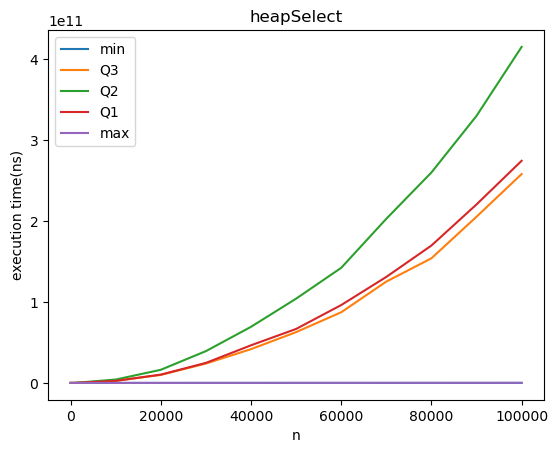
\includegraphics[scale = 0.8]{heapSelect.png}
    \caption{heapSelect时间复杂度}\label{heap}
\end{figure}
\begin{figure}
    \centering
    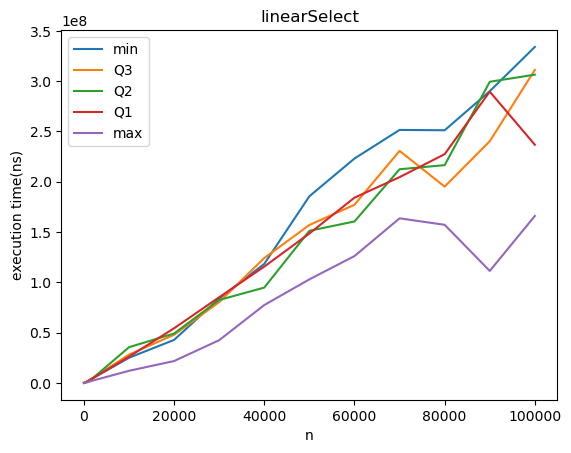
\includegraphics[scale = 0.8]{linearSelect.png}
    \caption{linearSelect时间复杂度}\label{linear}
\end{figure}
\begin{figure}
    \centering
    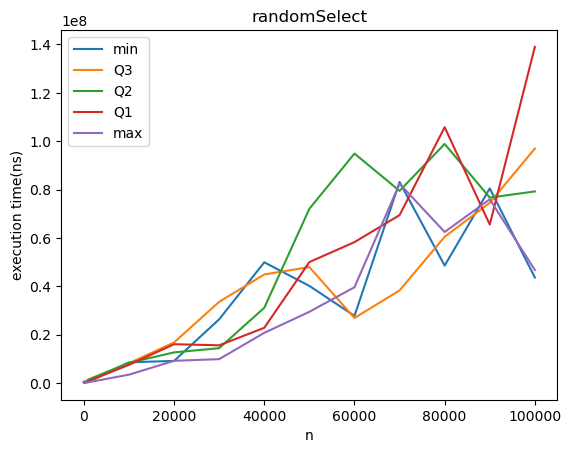
\includegraphics[scale = 0.8]{randomSelect.png}
    \caption{randomSelect时间复杂度}\label{random}
\end{figure}
\end{solution}
\newpage
\begin{problem}{动态规划}
   给定一列值$<v_1,v_2,\cdots,v_n>,v_i>0,i=1,\cdots,n$,求集合$\{1,2,\cdots,n\}$的一个二划分$\{A,B\}$,
   使得$\sum_{i\in B}v_i-\sum_{i\in A}v_i>0$且取最小值。输出分为4行,分别为
   \begin{enumerate}
    \item $\sum_{i\in A}v_i$
    \item A中元素(升序)
    \item $\sum_{i\in B}v_i$
    \item B中元素(升序)
   \end{enumerate}
   输入输出示例如下:
   
   Input:

   2 1 3 1 5 2 3 4

   Output:

   10

   1 3 5

   11 
   
   2 4 6 7 8
   
   要求首先通过暴力方法求解。
   然后使用动态规划方法进行求解,要求先从动态规划的角度对该题目进行分析,并写出递归属性。同时还应涉及
   用于存储中间量的数组。对于两种方式,都要求分析时间复杂度,并通过实验来检验分析结果。
\end{problem}
\begin{solution}
    暴力方法即枚举$\{1,2,\cdots,n\}$的所有可能的二划分。由于对于$i,1\leq i\leq n$,要么它属于$A$,要么它属于$B$,
    而这可以用0和1来表示。又因为当我们确定完所有元素的归属后,也就确定了一个划分,所以可以用长度为$n$的01串来编码划分。
    通过递增的方式来遍历所有长度为$n$的01串,并通过位运算将信息提取出来。遍历的01串数量为$2^n$,对于每个01串,
    要计算它对应的差值,需要$\Theta(n)$次计算,所以暴力方法的时间复杂度为$\Theta(n2^n)$,其中$n$为输出数组的长度。
    伪代码如下。

    \begin{function}
        \Return{(i>>j)$\&$1}\tcc*[h]{提取出第j位}
        \caption{extract(i,j)}
    \end{function}
    \begin{function}
        \SetKw{in}{in}
        A = []\;
        \For{j \in [0..n-1]}{
            \lIf{extract(i,j)==1}{A.append(j)}
        }
        \Return{A}
        \caption{extractSolution(i,n)}
    \end{function}
    \begin{algorithm}[H]
        \SetKw{len}{len}
        \SetKw{sum}{sum}
        \SetKw{in}{in}
        l = \len(values)\;
        MAX = 1<<l\tcp*[h]{所有长度为n的01串小于该值}\;
        i = 0\tcp*[h]{01串}\;
        ans = 0\tcp*[h]{记录最佳的01串}\;
        bestdiff = \sum(values)\tcp*[h]{记录最佳的差值}\;
        \While{i<MAX}
        {
            diff = 0\tcp*[h]{当前01串对应的差值}\;
            \For{j \in [0..l-1]}
            {
                \eIf(\tcp*[h]{提取出第j位}){
                    extract(i,j) == 1\;
                }
                {
                    diff -= values[j]
                }
                {
                    diff += values[j]
                }
            }
            \If(\tcp*[h]{更新最佳01串}){diff $\geq $0 and diff$<$bestdiff }
            {
                bestdiff = diff\;
                ans = i\;
            }
            i += 1\;
        }
        \Return{extractSolution(ans,l)}
        \caption{brute-force(values)}
    \end{algorithm}
我利用python语言完成了算法的实现。环境为:Python 3.11.7。

结果实验得到如下运行时间:

\begin{figure}[!h]
    \centering
 \begin{tabular}{c|c|c|c|c|c}
   输入长度$n$& 5  &  10& 15&20&25\\
   \hline 运行时间$(ns)$&   37100& 1202700& 56254000& 2161726300& 86466016500   \\
\end{tabular}   
\end{figure}

从图\ref{brute}可以看出,实验结果符合由分析得到的时间复杂度。

\begin{figure}
    \centering
    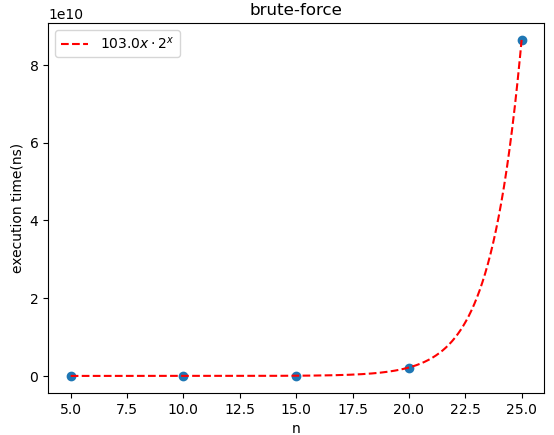
\includegraphics[scale = 0.6]{brute.png}
    \caption{暴力方法时间复杂度}\label{brute}
\end{figure}

想要使得差值$\sum_{i\in B}v_i-\sum_{i\in A}v_i$最小,等同于“使得
$\sum_{i}v_i-2\sum_{i\in A}v_i>0$或$\frac{1}{2}\sum_{i}v_i-\sum_{i\in A}v_i>0$最小”。
由于输入数组中的元素都是正整数,可以继续转换为“使得$\lfloor\frac{1}{2}\sum_{i\leq n}v_i\rfloor\geq\sum_{i\in A}v_i$
且$\sum_{i\in A}v_i$尽可能地大($A\subseteq\{1,2,\cdots,n\}$)”。

问题“使得$\sum_{i\in A}v_i\leq x$
且$\sum_{i\in A}v_i$尽可能地大($A\subseteq\{1,2,\cdots,y\}$)”的最优解对应的$\sum_{i\in A}v_i$记为$m[x,y]$,则有
\[m[i,j] = \begin{cases}
    m[i,j-1]&v_{j}>i\\
    \max \{m[i-v_j,j-1]+v_j,m[i,j-1]\}&else\\
\end{cases}\]
显然,当$v_j>i$时,m[i,j]中不可能包含$v_j$,因为这违反了不等式约束,从而m[i,j]与m[i,j-1]对应的合法的解相同,
最优解也相同,从而m[i,j]=m[i,j-1]。
当$v_j\leq i$时,由反证法易得,若$j\notin A$,则$A\subseteq\{1,2,\cdots,j-1\}$,对应的最优解为$m[i,j-1]$的最优解;若$j \in A$,则对应的最优解为$\{j\}\cup A^{\prime}$,
其中$A^{\prime}$对应$m[i-v_j,j-1]$的最优解。

 记$M = \lfloor\frac{1}{2}\sum_{i\leq n}v_i\rfloor$。原问题的最优解对应的和便是$m[M,n]$。想要计算得到$m[M,n]$,共需计算$M\cdot n$个值,所以时间复杂度为$\Theta(sn)$,
其中$s = \sum_{i=1}^{n}v_i$,$n$为输入元素的个数。

为了回溯还原最优解,需要保存过程中计算得到的$m[i,j]$值。回溯过程从m[M,n]开始,若$m[x,y]==m[x,y-1]$,则说明$m[x,y]$的最优解的构成和$m[x,y-1]$相同。
否则,说明$m[x,y]$对应的最优解中,$v_y\in A$,剩余部分由是$m[x-v_y,y-1]$对应的最优解。回溯过程所需要的时间复杂度为$\Theta(s+n)$

当$j=0$时,说明$m[i,j]$对应的最优解中$A=\varnothing$,所以$m[i,0]=0$。当$i=0$时,由于$v_k>0$,最优解中$A=\varnothing$,
从而$m[0,j]=0$。

伪代码以及实验结果如下,可以看出,实验结果符合由分析得出的时间复杂度。

\begin{figure}[!h]
    \centering
    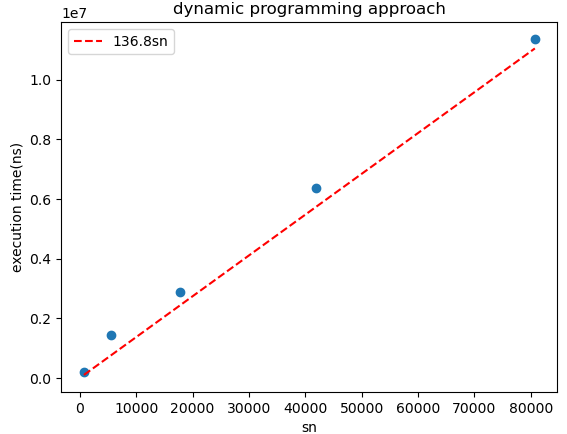
\includegraphics[scale = 0.6]{dynamic.png}
    \caption{动态规划方法时间复杂度}\label{dynamic}
\end{figure}

\begin{algorithm}[H]
    \SetKw{sum}{sum}
    \SetKw{max}{max}
    \SetKw{len}{len}
    \SetKw{in}{in}
    \SetKw{range}{range}
    \SetKw{break}{break}
    \tcp*[h]{values下标从1开始}\;
    M = $\lfloor$\sum(values)/2$\rfloor$\;
    l = \len(values)\;
    初始化一个(M+1)$\times$(l+1)的全零数组dp\;
    \For{i \in [1..M]}
    {
        \For{j \in [1..l]}
        {
            \eIf{values[j]>i}
            {
                dp[i][j] = dp[i][j-1]\;
            }{
                dp[i][j] = max(dp[i][j-1],dp[i-values[j]][j-1]+values[j])
            }
        }
    }
    A=[]\tcp*[h]{开始回溯}\;
    x = M\;
    y = l\;
    \While{
        x and y
    }
    {
        \lWhile{y and dp[x][y] == dp[x][y-1]}
        {
            y -= 1
        }
        \lIf{y==0}{\break}
        A.append(y)\;
        x -= values[y-1]\;
        y -= 1\;
    }
    \Return{A}
    \caption{DynamicProgrammingApproach(values)}
\end{algorithm}
% 对于该问题的一个最优解,其中$A=\{i_1,i_2,\cdot,i_r\},i_1<i_2<\cdots<i_r$,
% $A^{\prime}=\{i_1,i_2,\cdot,i_{r}\}\backslash\{n\}$也构成问题
% “使得$\lfloor\frac{1}{2}\sum_{i\leq n-1}v_i\rfloor\geq\sum_{i\in A^{\prime}}v_i$
% 且$\sum_{i\in A^{\prime}}v_i$尽可能地大($A^{\prime}\subseteq\{1,\cdots,n-1\}$)”的最优解。事实上,如果
% $A^{\prime\prime}\neq A^{\prime}$在该子问题上比$A^{\prime}$更优,那么显然$A^{\prime\prime}\cup\{i_r\}$在原问题上
% 比$A=A^{\prime}\cup\{i_r\}$还要优,从而产生矛盾。因此该问题具有最优子结构性质,可以采用动态规划方法解决。

% 记“使得$\lfloor\frac{1}{2}\sum_{i\leq n}v_i\rfloor\geq\sum_{i\in A}v_i$
% 且$\sum_{i\in A}v_i$尽可能地大($A\subseteq\{1,2,\cdots,n\}$)”的最优解为$A_n$。显然,
% 如果$v_n$
\end{solution}
\end{document}